%%%%%%%%%%%%%%%%%%%%%%%%%%%%%%%%%%%%%%%%%%%%%%%%%%%%%%%%%%%%%%%%%%%%%%%
%% Vorlage f�r Abschlussarbeiten                                     %%
%%-------------------------------------------------------------------%%
%% Datei:        appendix.tex                                        %%
%% Beschreibung: Weitere Informationen, Schaltpl�ne und Quelltext    %%
%% Autor: 			 Stefan Herrmann                                     %%
%% Datum:        03.12.2012                                          %%
%% Version:      1.0.1                                               %%
%%%%%%%%%%%%%%%%%%%%%%%%%%%%%%%%%%%%%%%%%%%%%%%%%%%%%%%%%%%%%%%%%%%%%%%
\appendix
\chapter{Quellcode}
\index{Quellcode}
\lstinputlisting[language=C++, caption={move\_group\_interface.cpp}]{images/results/move_group_interface.cpp}
\lstinputlisting[language=C++, caption={gesture\_control.cpp}]{images/results/gesture_control.cpp}


\chapter{Arbeitsaufwand}
\index{Arbeitsaufwand}

\begin{figure}[H]
	\centering
		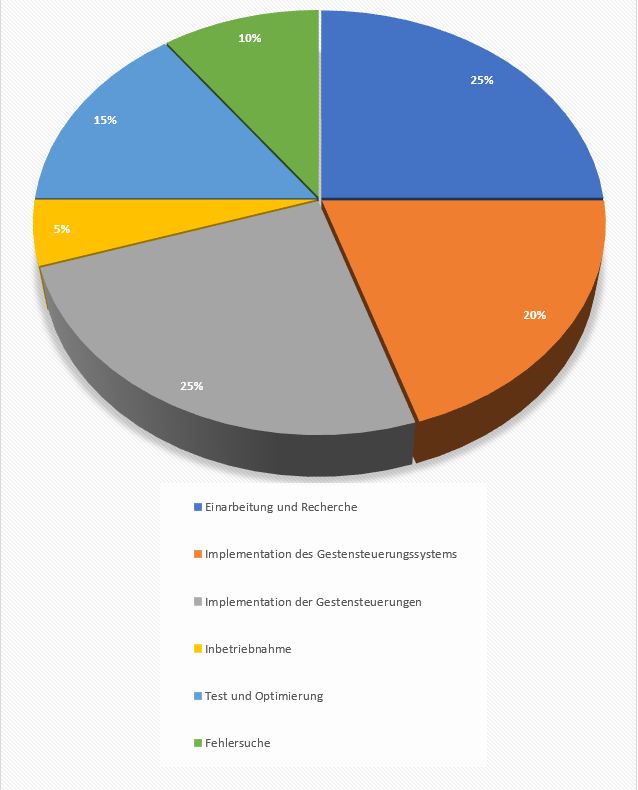
\includegraphics{images/appendix/DiagrammArbeitsaufwand.png}
	\caption{Arbeitsaufwand}
	\label{fig:arbeitsaufwand}
\end{figure}




